% FILE: figures/evolution_operator.tex
% Evolution operator E: K(t) -> K(t+dt)

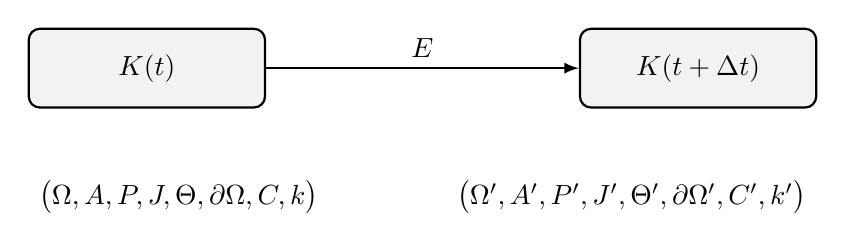
\begin{tikzpicture}[>=latex,thick]
  \node[draw, rounded corners, fill=gray!10, minimum width=3cm, minimum height=1cm] (Kt)   at (0,0) {$K(t)$};
  \node[draw, rounded corners, fill=gray!10, minimum width=3cm, minimum height=1cm] (Ktdt) at (7,0) {$K(t+\Delta t)$};

  \draw[->] (Kt) -- node[above] {$E$} (Ktdt);

  % Annotations
  \node[anchor=north west] at (-1.5,-1.3) {$\big(\Omega,A,P,J,\Theta,\partial\Omega,C,k\big)$};
  \node[anchor=north east] at (8.5,-1.3) {$\big(\Omega',A',P',J',\Theta',\partial\Omega',C',k'\big)$};
\end{tikzpicture}


